%---
\section{Introduction}\label{sec:intro}\label{sec:introduction}
\dsf\ is a Liquid Argon Time Projection Chamber (\lar\ \tpc), operated in Italy's Gran Sasso National Laboratory (LNGS) to search for nuclear recoils induced by weakly interacting massive particles (WIMPs). The first physics result was reported in \cite{Agnes:2015gu} based on 50 live data collection days with Atmospheric Argon (AAr). It provides the most sensitive limit on a dark matter search using a \lar\ \tpc\ to date with a 90\% CL upper limit on the WIMP-nucleon spin-independent cross section of $6.1 x 10^{-44}$ cm$^2$ for a WIMP mass of 100 GeV/c$^2$.  %along with two other key results: ar bg can be suppressed for ton-scale experiments using \uar and efficiency of the veto 

A first WIMP search using argon extracted from underground sources (Underground Argon, UAr) has been reported in \cite{Agnes:2015_uar}, following the WIMP search with AAr. UAr has a lower concentration of the radioactive $\beta$-emitter $^{39}$Ar by a factor (1.4 $\pm$ 0.2) $\times\, 10^3$ relative to AAr. Calibration campaigns have been performed in the presence of AAr and UAr.

The \dsf\ apparatus is described in detail in \cite{Agnes:2015gu}. As shown in fig.~\ref{fig:wholeAssembly_insideDetectors}, it features a \lar\ \tpc\ surrounded by a 30 t liquid scintillator-based veto (LSV) system, placed inside a water Cherenkov veto detector (\wcv), both of which measure in-situ and suppress radiogenic and cosmogenic backgrounds \cite{Agnes:2015qyz}. On the top of the \wcv\ is a radon-free clean room (CRH for Clean Room Hanoi) housing the cryogenic supply system and electronics (Fig.~\ref{fig:DS50_with_CALIS}). The \lsv\ may be accessed through one of four gate valves in CRH, which are approximately 6 m above the center of the LSV. Each gate valve connects to an access port, called organ pipe, 15 cm in diameter which leads through the WCV and opens into the LSV, 80 cm off the TPC's vertical z-axis.
%=6145=70+120+400+3455+20+251+1372+457 from http://darkside-docdb.fnal.gov:8080/cgi-bin/RetrieveFile?docid=858&filename=NoFlyZone-DS50_vers02.pdf&version=14

%After this introduction the CALIS design requirements and hardware realization are described in Sec.~\ref{sec:hardware}. Calibration campaigns and some of their physics highlights are discussed in Sec.~\ref{sec:CalibCampaigns}, before concluding in Sec.~\ref{sec:Conclusion}.

\begin{figure}[htbp]
 \centering
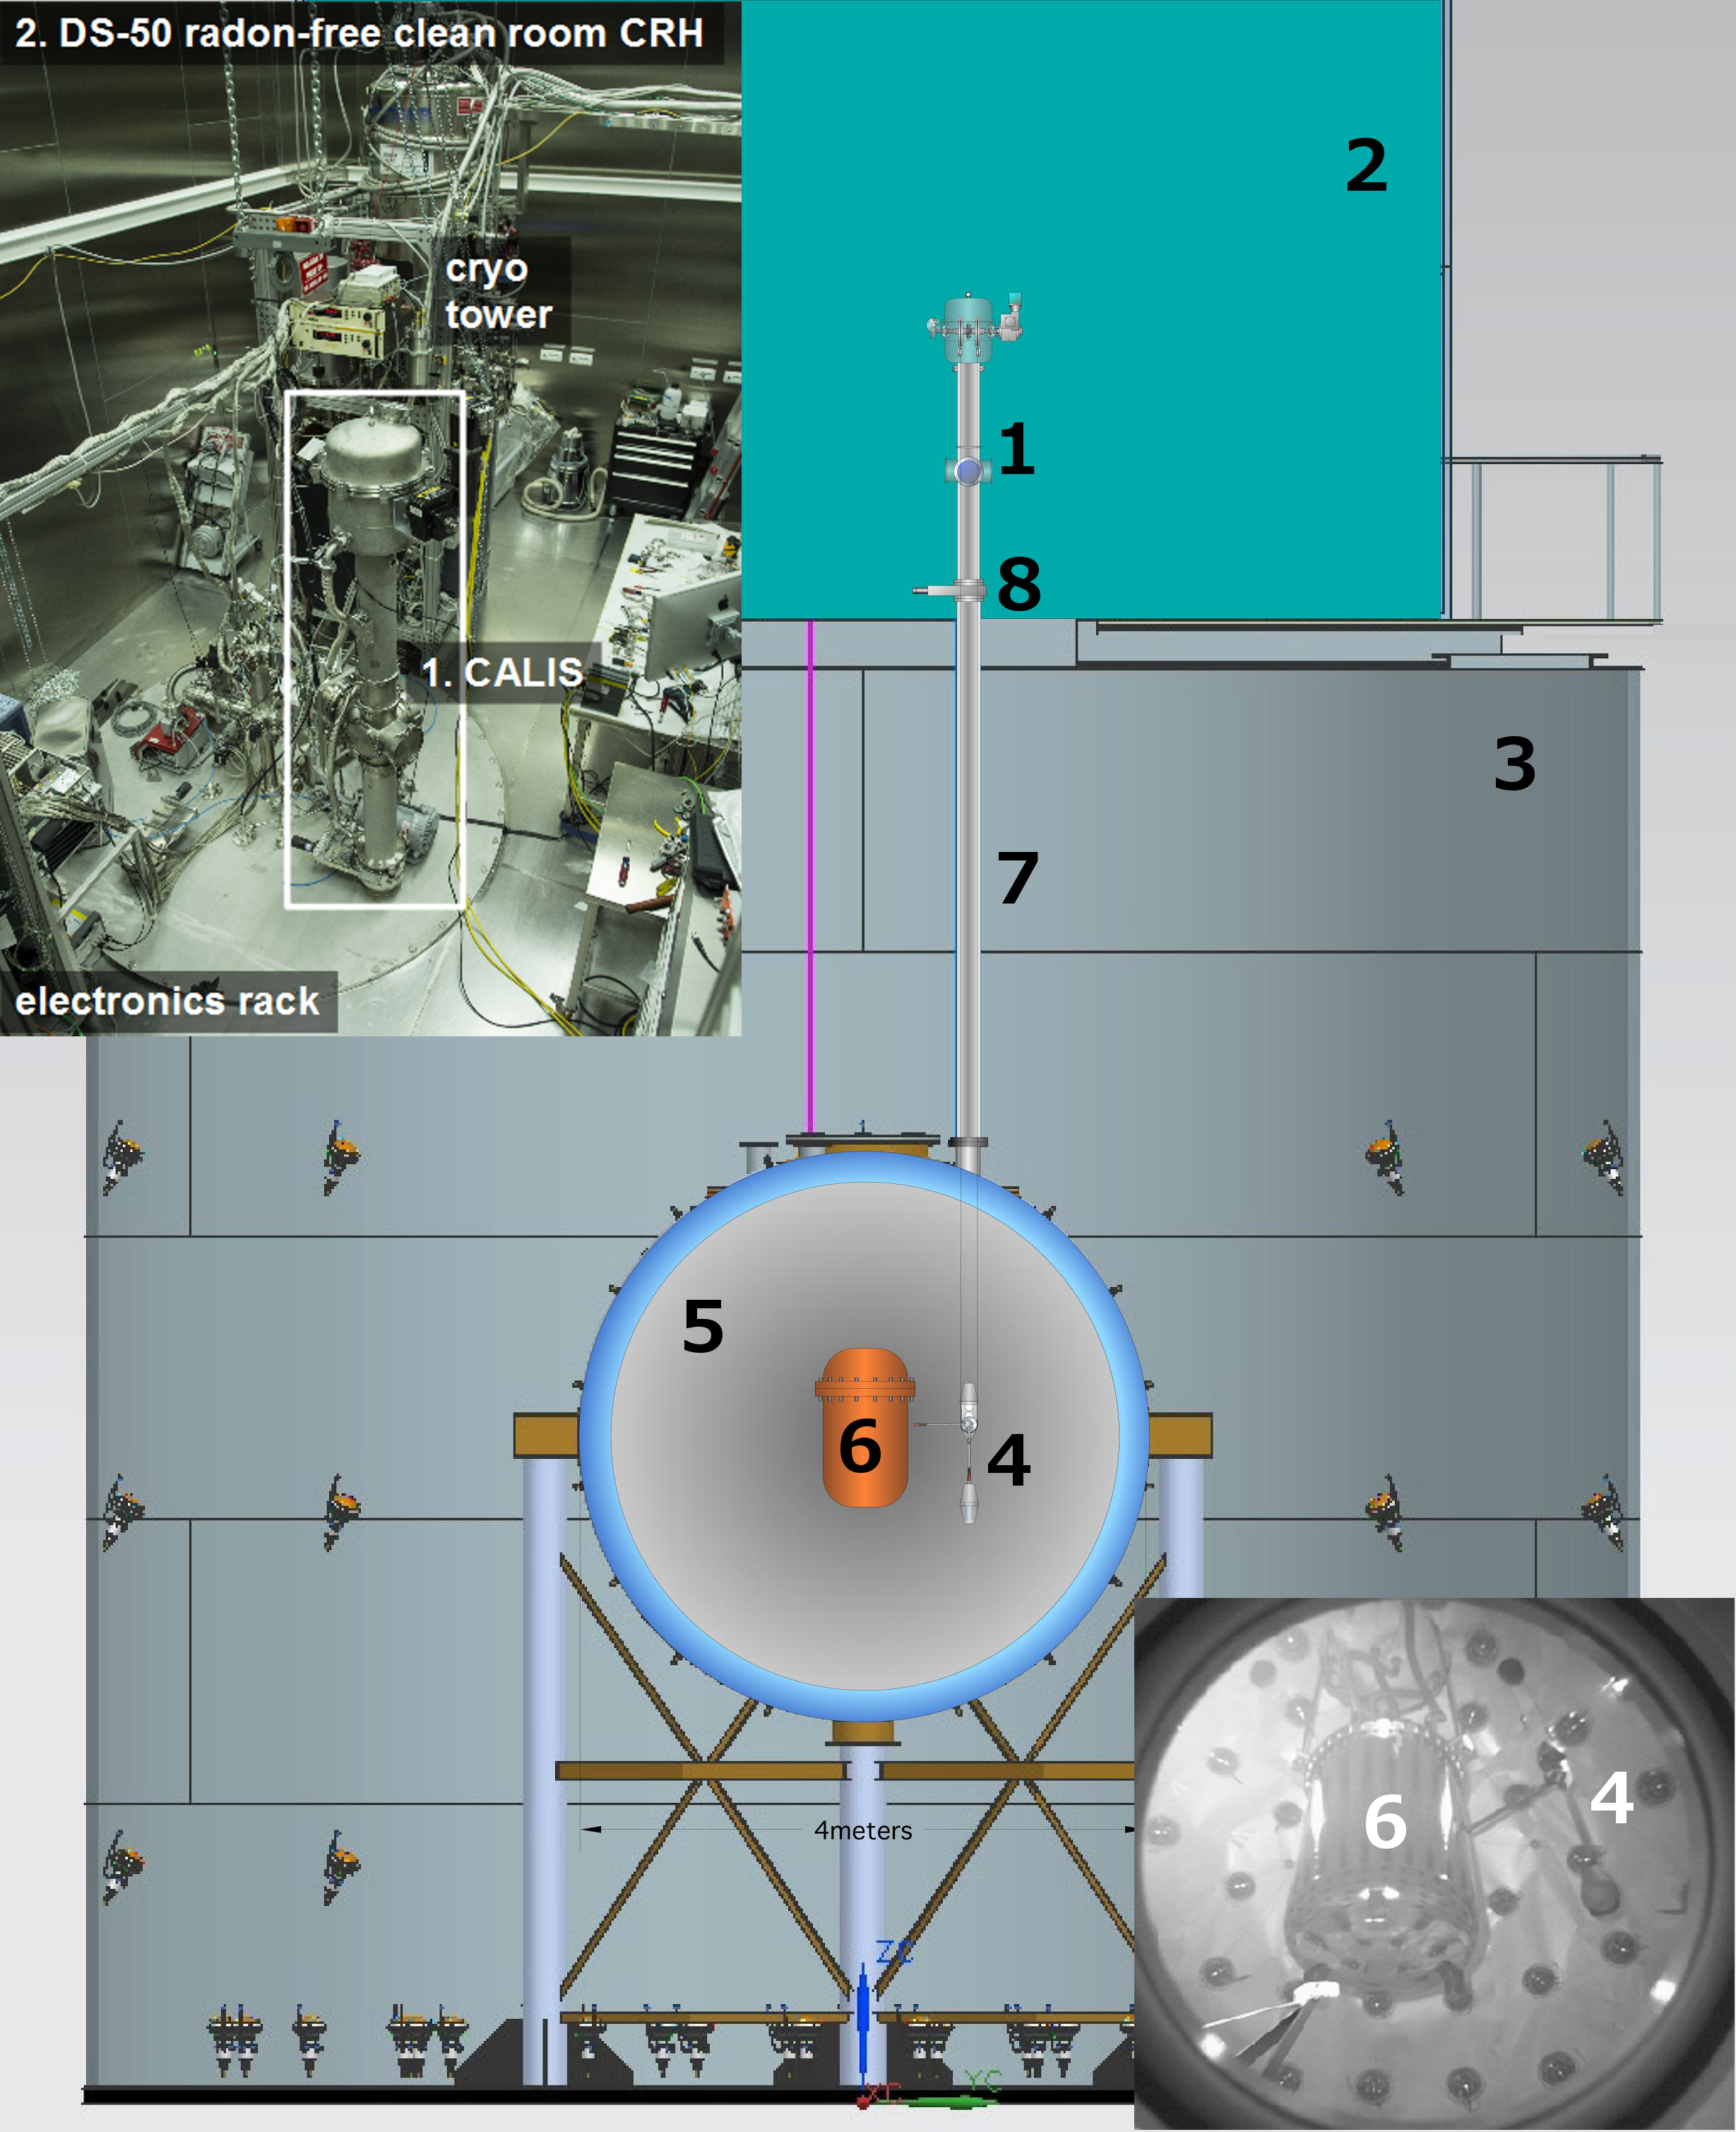
\includegraphics[width=\textwidth]{Figures/DS50_with_CALIS_twoinsets}
\caption{A conceptual drawing of CALIS (1) installed in the radon-free clean room, CRH (2), atop the water Cherenkov veto (\wcv, 3). The deployment device (4) which contains the source is deployed in the liquid scintillator veto (LSV, 5) next to the liquid argon time projection chamber's (\lar\ \tpc) cryostat (6). The clean room and the LSV are connected through four access ports, called organ pipes (only one of which is drawn in the above sketch (7)). All four organ pipes end in CRH at gate valves (8) which can be manually opened or closed. During normal operations all four organ pipes are closed. Not included in the drawing are tubes connecting the cryogenic systems in CRH to the cryostat in the \lsv. The top left inset shows CALIS after successful installation inside CRH. The bottom right inset shows a photograph taken with a camera looking upwards into the \lsv\ from the bottom. The deployment device's source arm is articulated and the source in its tip is next to the \lar\ \tpc's cryostat. (The numbering in the insets matches the drawing's.) \label{fig:wholeAssembly_insideDetectors}\label{fig:DS50_with_CALIS}}
\end{figure}